% ****************************************************************************************************
\chapter{Business Models of Platform as a Service Providers -- Current State}\label{ch:sota}
% ****************************************************************************************************

In order to assess the current state of \ac{PaaS} providers' business models and identify key elements within these business models, the current business models of 23 \ac{PaaS} providers were analyzed. The initial selection of the analyzed \ac{PaaS} providers in this thesis was based on technical reports respectively market reports provided by three different market research companies:
\begin{itemize}
	\item Forrester Research, Inc. -- \citet{Ried2011a,Rymer2011}
	\item \ac{IDC} -- \citet{Bradshaw2012,Hendrick2012, Hendrick2012a}
	\item Gartner, Inc. -- \citet{Smith2012}
\end{itemize}
The initially identified and selected \ac{PaaS} providers were further selected to receive a manageable set of representative \ac{PaaS} providers. Four disjunct selection criteria were used in the second evaluation round to identify the final set of 23 \ac{PaaS} providers -- market share, growth rate, availability of the platform to customers as of February 2013, and background of the \ac{PaaS} provider, for instance, former purely \ac{IaaS} or \ac{SaaS} providers extend their cloud portfolio with \ac{PaaS} functionalities. According to \citet{Hendrick2012}, the world largest \ac{PaaS} provider is GXS Worldwide, Inc. (cf. Appendix \ref{ch:app01:gxs}) with a market share of 14.2\% in 2011 and with a growth rate of 428.6\% in 2011 CloudBees (cf. Section \ref{ch:sota:cb}) is the fastest-growing \ac{PaaS} provider.

In the following, four case studies -- CloudBees, GigaSpaces Cloudify, Facebook Developers, and SAP NetWeaver Cloud -- are described in detail. The remaining 19 case studies are presented for reasons of comprehensibility within Appendix \ref{ch:app01}. To receive a coherent representation, all presented business models within this thesis follow the prior introduced business model conceptualization approach (cf. Section \ref{ch:sota:bmc}).

Based upon the performed analyzes of current \ac{PaaS} providers' business models, a classification model for \ac{PaaS} providers is developed and introduced in Section \ref{ch:sota:cm}.

\section{Classification Scheme}\label{ch:sota:cm}

"Classification in an important tool for perception, because it provides clarity. \ldots Well-known examples are the periodic table of the elements in chemistry \ldots and the decimal classification in library science." \citep[p. 36]{Fettke2003}. In order to achieve this objective, the classification methodology introduced by \citet{Fettke2003} is used to develop a classification scheme for \ac{PaaS} business models. According to \citet[p. 39]{Fettke2003}, "A classification scheme consists of a set of characteristics which are suitable to classify objects of a specific application domain." Within each classification process, the crucial step is to select the appropriate classification objects and characteristics, neither too general nor too specific. The following six universal guidelines are helpful to improve the quality of classification schemes -- completeness, precision, consistency, extensibility, user-friendliness, and economic efficiency \citep[pp. 40-41]{Fettke2003}. 

Five interrelated phases which are performed subsequently and possibly iterative constitute the proposed classification methodology (cf. Figure \ref{fig:cm}) -- (1) Inception, (2) Elaborate Characteristics, (3) Specify Classification Scheme, (4) Test, and (5) Use and Maintenance. These five phases were applied as follows:

\begin{figure}[htb]
	\centering
	% ****************************************************************************************************
% Classification Procedural Model
% ****************************************************************************************************

\begin{tikzpicture}[scale=0.75, every node/.style={scale=0.75}]

\node[draw,text width=7em,text centered,rectangle,rounded corners,minimum height=4em,thick] (1) at (5,5.5) {(1) Inception};
\node[draw,text width=7em,text centered,rectangle,rounded corners,minimum height=4em,thick] (2) at (9,3) {(2) Elaborate Characteristics};
\node[draw,text width=7em,text centered,rectangle,rounded corners,minimum height=4em,thick] (3) at (8,0) {(3) Specify Classification Scheme};
\node[draw,text width=7em,text centered,rectangle,rounded corners,minimum height=4em,thick] (4) at (2,0) {(4) Test};
\node[draw,text width=7em,text centered,rectangle,rounded corners,minimum height=4em,thick] (5) at (1,3) {(5) Use and Maintenance};

\path 
	(1.east) edge [->,thick,>=stealth'] (2.north)
	(2.south) edge [->,thick,>=stealth'] (3.north)
	(3.west) edge [->,thick,>=stealth'] (4.east)
	(4.north) edge [->,thick,>=stealth'] (5.south)
	(5.north) edge [->,thick,>=stealth'] (1.west);

\end{tikzpicture}
	\caption[Classification Methodology]{Classification Methodology adapted from \citet{Fettke2003}}
	\label{fig:cm}
\end{figure}

\begin{enumerate}
	\item Inception: For the purpose of classifying \ac{PaaS} business models, a corresponding \ac{PaaS} classification scheme needs to be developed. This scheme should further serve as a starting point for the later introduced interdependencies within \ac{PaaS} business models (cf. Chapter \ref{ch:dm}).

	\item Elaborate Characteristics: The data obtained through the comprehensive analysis of existing \ac{PaaS} business models was analyzed on the one hand as stand-alone business models (analyzing within-case data) and on the other hand to search for cross-case patterns \citep[pp. 539-540]{Eisenhardt1989}. Within the identification process of potential cross-case patterns two different approaches were used. First, the four elements of a business model representation (cf. Section \ref{ch:sota:bmc}) introduced by \citet{Johnson2008} were used to compare business models and reveal common similarities as well as fundamental varieties. Second, various selective pairs of two business models were built to uncover further potential distinguishing features. 

	\item Specify Classification Scheme: In order to visualize the identified \ac{PaaS} business model categories as well as their characteristics in a structured approach, the concept of a morphological matrix adapted from \citet{ Zwicky1969} was used (cf. Figure \ref{fig:cs}).

	\item Test: By classing the set of 23 investigated \ac{PaaS} providers business models, the classification scheme was evaluated and iteratively revised as well as enhanced. Whereas classing is considered "as an operation whereby objects \ldots are assigned to classes \ldots which have been previously defined" \citep[p. 130]{Marradi1990}.

	\item Use and Maintenance: The finally obtained \ac{PaaS} business model classification scheme (cf. Figure \ref{fig:cs}) was used to survey the 23 investigated \ac{PaaS} providers business models (cf. Appendix \ref{ch:app02}) and as a basis to answer the research question: "How should \ac{PaaS} business models be designed?" (cf. Chapter \ref{ch:dm}).

\end{enumerate}





\begin{figure}[htb]
	\centering
	% ****************************************************************************************************
% Classification Scheme
% ****************************************************************************************************

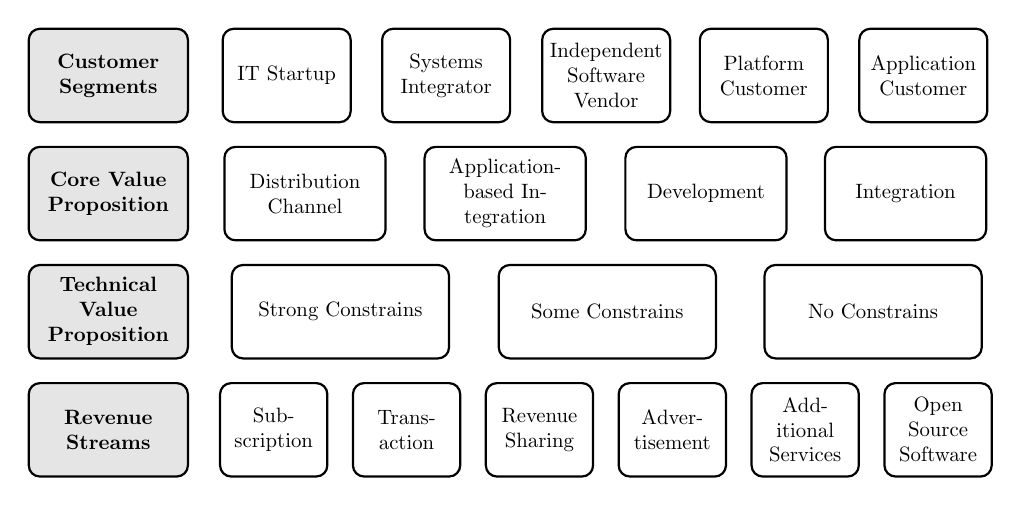
\begin{tikzpicture}[scale=0.75, every node/.style={scale=0.75}]

\node[font={\bfseries},draw,text width=7em,text centered,rectangle,rounded corners,minimum height=4.5em,thick,fill=gray!20] (1) at (0,6) {Customer Segments};
\node[font={\bfseries},draw,text width=7em,text centered,rectangle,rounded corners,minimum height=4.5em,thick,fill=gray!20] (1) at (0,4) {Core Value Proposition};
\node[font={\bfseries},draw,text width=7em,text centered,rectangle,rounded corners,minimum height=4.5em,thick,fill=gray!20] (1) at (0,2) {Technical Value Proposition};
\node[font={\bfseries},draw,text width=7em,text centered,rectangle,rounded corners,minimum height=4.5em,thick,fill=gray!20] (1) at (0,0) {Revenue Streams};

\node[draw,text width=5.5em,text centered,rectangle,rounded corners,minimum height=4.5em,thick] (1) at (3.02,6) {IT Startup};
\node[draw,text width=5.5em,text centered,rectangle,rounded corners,minimum height=4.5em,thick] (1) at (5.72,6) {Systems Integrator};
\node[draw,text width=5.5em,text centered,rectangle,rounded corners,minimum height=4.5em,thick] (1) at (8.43,6) {Independent Software Vendor};
\node[draw,text width=5.5em,text centered,rectangle,rounded corners,minimum height=4.5em,thick] (1) at (11.1,6) {Platform Customer};
\node[draw,text width=5.5em,text centered,rectangle,rounded corners,minimum height=4.5em,thick] (1) at (13.8,6) {Application Customer};

\node[draw,text width=7.1em,text centered,rectangle,rounded corners,minimum height=4.5em,thick] (1) at (3.33,4) {Distribution Channel};
\node[draw,text width=7.1em,text centered,rectangle,rounded corners,minimum height=4.5em,thick] (1) at (6.72,4) {Application-based Integration};
\node[draw,text width=7.1em,text centered,rectangle,rounded corners,minimum height=4.5em,thick] (1) at (10.12,4) {Development};
\node[draw,text width=7.1em,text centered,rectangle,rounded corners,minimum height=4.5em,thick] (1) at (13.5,4) {Integration};

\node[draw,text width=9.8em,text centered,rectangle,rounded corners,minimum height=4.5em,thick] (1) at (3.93,2) {Strong Constrains};
\node[draw,text width=9.8em,text centered,rectangle,rounded corners,minimum height=4.5em,thick] (1) at (8.45,2) {Some Constrains};
\node[draw,text width=9.8em,text centered,rectangle,rounded corners,minimum height=4.5em,thick] (1) at (12.95,2) {No Constrains};

\node[draw,text width=4.5em,text centered,rectangle,rounded corners,minimum height=4.5em,thick] (1) at (2.8,0) {Sub-scription};
\node[draw,text width=4.5em,text centered,rectangle,rounded corners,minimum height=4.5em,thick] (1) at (5.05,0) {Trans-action};
\node[draw,text width=4.5em,text centered,rectangle,rounded corners,minimum height=4.5em,thick] (1) at (7.3,0) {Revenue Sharing};
\node[draw,text width=4.5em,text centered,rectangle,rounded corners,minimum height=4.5em,thick] (1) at (9.55,0) {Adver-tisement};
\node[draw,text width=4.5em,text centered,rectangle,rounded corners,minimum height=4.5em,thick] (1) at (11.8,0) {Add-itional Services};
\node[draw,text width=4.5em,text centered,rectangle,rounded corners,minimum height=4.5em,thick] (1) at (14.05,0) {Open Source Software};

%\node [node, right of=1] (2) {map};

%\node[draw,text width=7em,text centered,rectangle,rounded corners,minimum height=4em,thick] (10) {Customer Segments};
%\node[draw,text width=7em,text centered,rectangle,rounded corners,minimum height=4em,thick,below of=10] (20) {Core Value Proposition};
%\node[draw,text width=7em,text centered,rectangle,rounded corners,minimum height=4em,thick,below of=20] (30) {Technical Value Proposition};
%\node[draw,text width=7em,text centered,rectangle,rounded corners,minimum height=4em,thick,below of=30] (40) {Revenue Streams};

%\node[draw,text width=7em,text centered,rectangle,rounded corners,minimum height=4em,thick,right of=40] (41) {Subscription};
%\node[draw,text width=7em,text centered,rectangle,rounded corners,minimum height=4em,thick,right of=41] (42)  {Transaction};
%\node[draw,text width=7em,text centered,rectangle,rounded corners,minimum height=4em,thick,right of=42] (43) {Revenue Sharing};
%\node[draw,text width=7em,text centered,rectangle,rounded corners,minimum height=4em,thick,right of=43] (44)  {Advertisement};
%\node[draw,text width=7em,text centered,rectangle,rounded corners,minimum height=4em,thick,right of=44] (45)  {Additional Services};
%\node[draw,text width=7em,text centered,rectangle,rounded corners,minimum height=4em,thick,right of=45] (46)  {Open Source Software};

\end{tikzpicture}
	\caption{PaaS Business Model Classification Scheme}
	\label{fig:cs}
\end{figure}



\section{The Case of CloudBees}\label{ch:sota:cb}

CloudBees was founded in the beginning of 2012 and introduced its identically named \ac{PaaS} offer. Many of CloudBees' management team members, including the founder, worked prior for companies like Oracle, Sun, IBM, and VMware or were involved in development projects around JBoss and Jenkins CI. Already the background of CloudBees' management reveals the main objective -- a \ac{PaaS} solution truly dedicated around the Java programming language ecosystem, supporting the whole application lifecycle \citep{CloudBees2013}.

The CloudBees platform is composed of two distinct but related concepts. First, all development, integration, and testing tasks are performed within the DEV@cloud. Core of this part of the platform is the Jenkins Continuous Integration server. Once an application is ready to go live, the application is migrated to the RUN@cloud. Basically, the RUN@cloud represents a traditional application server, including the functionalities load balancing, scalability, and high availability, based on various cloud infrastructures.

Mainly two different customer groups are attracted by CloudBees platform solution -- business end-consumer and \acp{ISV}. The first-mentioned group utilizes the platform to manage the entire application lifecycle -- including development, quality assurance and testing, deployment and release management, as well as monitoring and administration. Due to the fact, that all applications upon the CloudBees platform are based on standard Java and not on specific CloudBees \acp{API}, potential customers are not faced with a so called lock-in effect. Moreover, platform customers can select between multi-tenant and dedicated RUN@cloud's. In case of dedicated instances, they can choose the appropriate cloud infrastructure -- private, public, and hybrid provisioning scenarios are supported. Via the CloudBees Partner Ecosystem, business end-consumer can purchase third-party applications and services and extend the CloudBees platform functionalities. 

Platform extensions are provided by the second customer group, the \acp{ISV}. CloudBees uniquely defined mission -- support the whole application lifecycle for standard Java and \ac{JVM} based applications within the cloud -- enables \acp{ISV} to expand the already existing platform capabilities by deployment and testing tools, comprehensive monitoring features, as well as different databases. All third-party applications, tools, and services are listed within the CloudBees Partner Ecosystem. Especially for small \acp{ISV}, but certainly also for all other \acp{ISV}, it is beneficial, that the payment handling, inclusive billing, for third-party extensions is performed by CloudBees.

The overall revenue of CloudBees is composed of two revenue streams -- through CloudBees' partners and CloudBees' platform customers. Consulting partners, i.e. \acp{SI}, need to pay an annual partner fee -- silver partners USD 2.000 and gold partners USD 5.000 -- to become a certified \linebreak CloudBees Service Partner. For all third-party applications, tools, and services provided by \acp{ISV}, denoted by CloudBees as Technology Partners, CloudBees gets a default revenue share of 30\%. Nevertheless, CloudBees offers the possibility to negotiate the revenue share rate individually.

Business end-consumer pay for the CloudBees platform a combination of subscription and transaction based fees. The DEV@cloud is available as four different packages -- Free USD 0, Base USD 15, Pro USD 50, and Enterprise USD 100, all prices per month -- including different features and quotas. A different number of build minutes is included within all packages and additional build minutes can be purchased for USD 0.106 respectively 0.425 per hour. A multi-tenant RUN@cloud is either free (no additional features or services can be purchased) or charged per hour, based on the select application server and SSL connections. As mentioned above, the dedicated RUN@cloud can basically be hosted at any cloud infrastructure, with the result that a vast number of pricing models is possible. For instance, the CloudBees RUN@cloud platform hosted at \ac{AWS} infrastructure is priced between USD 153 - 644 per instance monthly. Furthermore, CloudBees is offering also a MySQL database which is priced based on the selected RUN@cloud \citep{CloudBees2013}.
\newpage
% ****************************************************************************************************
% Business Model CloudBees
% ****************************************************************************************************
\begin{longtable}{|L{\column}|L{\column}|L{\column}|L{\column}|}
	
	\hline
	\multicolumn{4}{|l|}{\textit{\nameref{bm:cloudbees}}}\\ 
	\hline
	\endfirsthead
	\hline  
	\multicolumn{4}{|l|}{\textit{continued from previous page (\nameref{bm:cloudbees})}}\\ 
	\hline
	\endhead
	\hline
	\multicolumn{4}{|r|}{\textit{continued on next page}}\\
	\hline
	\endfoot
	\hline
	\caption[Business Model CloudBees]{Business Model CloudBees \citep{CloudBees2013}}
	\label{bm:cloudbees}
	\endlastfoot
	
	\multicolumn{4}{|c|}{\large \textbf{Customer Value Proposition (CVP)}}\\ \hline
	
	\textbf{Target customer} &
	\textbf{Job to be done} &
	\multicolumn{2}{|L{\columnT}|}{\textbf{Offering}} \\ \hline
	
	% START CUSTOMERS
	\small
	Business End-Consumer &
	\small
	Manage the entire Java application lifecycle within the cloud in a cost efficiency manner & 
	\multicolumn{2}{|L{\columnT}|}{
	\vspace{-5mm}
	\small
	\begin{itemize}[leftmargin=*, parsep=0pt, topsep=0pt, itemsep=0pt]
				\item Manage the entire Java and \ac{JVM} application lifecycle
				\item CloudBees Eclipse plugin and \ac{SDK}
				\item Different deployment scenarios: public, private, and hybrid
				\item 'No vendor lock-in' (standard Java)
				\item CloudBees partner ecosystem provides platform extensions -- databases, monitoring as well as deployment tools\vspace{-\baselineskip} 
		\end{itemize}
	} \\ \hline
	\small	
	\ac{ISV} &
	\small
	Develop, manage, and market application lifecycle related applications and services globally &
	\multicolumn{2}{|L{\columnT}|}{
		\vspace{-5mm} 
		\small
		\begin{itemize}[leftmargin=*, parsep=0pt, topsep=0pt, itemsep=0pt]
				\item CloudBees platform as a service truly dedicated to Java and \ac{JVM} applications (clear mission)
				\item Service resp. application listing within the Ecosystem Technology Partner directory
				\item Support mechanism between CloudBees and service provider, to resolve customer problems within a narrow time frame
				\item Joint marketing activities
				\item Payment handling (incl. billing) by CloudBees\vspace{-\baselineskip} 
		\end{itemize}
	} \\ \hline

% END CUSTOMERS

% KEY RESOURCES
\multicolumn{2}{|L{\columnT}|}{\large \textbf{Key Resources}
\small
\begin{itemize}[leftmargin=*, parsep=0pt, topsep=0pt, itemsep=0pt]
				\item CloudBees' platform, including
					\begin{itemize}[leftmargin=*, topsep=0pt, itemsep=0pt]
						\item Build: create, integrate, and test
						\item Run: choose, deploy, and store
						\item Manage: scale, monitor, and enhance
					\end{itemize}
				\item CloudBees Eclipse plugin and \ac{SDK}
				\item Consulting partners, for instance Black Diamond Software
				\item Partnership with \ac{IaaS} providers, for instance \ac{AWS}\vspace{-\baselineskip} 
	\end{itemize}
} &
% KEY PPROCESSES
\multicolumn{2}{|L{\columnT}|}{\large \textbf{Key Processes}
\small
\begin{itemize}[leftmargin=*, parsep=0pt, topsep=0pt, itemsep=0pt]
				\item Maintain full lifecycle support for Java and \ac{JVM} applications as well as keep the platform up to date (in respect of new Java versions and features)
				\item Facilitate different deployment scenarios -- public, private, and hybrid -- based on multiple \ac{IaaS} providers
				\item Maintain partnerships with existing \ac{IaaS} providers as well as begin negotiations with potential providers
				\item Partner program for consulting partners, including business and marketing support, access to products plans, trainings, reselling options, and listing in the CloudBees Service Partner Directory
				\item Offer support via Stack Overflow, \ac{FAQ}, and documentation/ guides deployment tools\vspace{-\baselineskip} 
\end{itemize}
} \\ \hline

% PROFIT FORMULA
\multicolumn{4}{|L{\columnF}|}{\large \textbf{Profit Formula}
	\small
	\begin{itemize}[leftmargin=*, parsep=0pt, topsep=0pt, itemsep=0pt]
				\item Subscription and transaction based revenue for platform usage:
					\begin{itemize}[leftmargin=*, topsep=0pt, itemsep=0pt]
						\item DEV@cloud: USD 0 - 100 / Monthly + build minutes
						\item RUN@cloud Multi-Tenant: Free (limited) or transaction based (depends among other things on the used software stack per app per hour) 
						\item RUN@cloud Dedicated: Different IaaS providers, e.g. \ac{AWS} US m1.small USD 153 \/ Monthly
						\item Database: Offered by CloudBees (MySQL) USD 0 - 25 / Monthly or by different partners
					\end{itemize}
				\item Partner program fee: USD 2000 - 5000 / Yearly
				\item Revenue sharing (30\%; or individual negotiated) for applications and services offered by third parties\vspace{-\baselineskip} 
	\end{itemize}
} \\

\end{longtable}





\section{The Case of GigaSpaces Cloudify}\label{ch:sota:gsc}

Within the evolving \ac{PaaS} ecosystem are just a few open source platform solutions available -- Cloudify is one of them. Since the beginning of 2012, the Cloudify Open \ac{PaaS} Stack is available on the market. Cloudify itself and the Cloudify Community are promoted by the company GigaSpaces \citep{GigaSpaces2013a}.

The basic concept of Cloudify is the so-called external blueprint, also named as recipe. Within a blueprint the deployment and post-deployment activities of an application are described. This concept enables developers to migrate existing applications to cloud infrastructure without the need to adopt or change the source code. Moreover, based on the blueprint concept, applications can be deployed at or migrate between private, public, or even hybrid cloud infrastructures \citep{GigaSpaces2013a}.

Two distinct customer groups can use the Cloudify platform offer: (1) business end-consumers who want to move existing non-cloud applications to the cloud or develop and operate cloud applications and (2) \acp{ISV} who want to offer migration services (migrate on-premise applications onto cloud infrastructure). The value proposition for these two stakeholder groups include the promise to move any application without code or application architecture changes to the cloud, develop the external blueprint for an application once and be able to deploy the application at different cloud infrastructures, as well as full control over the Cloudify Open \ac{PaaS} Stack. Furthermore, an interactive shell and web-based user-interface for monitoring purposes are provided \citep{GigaSpaces2013a}.

As usual for many open source projects, a flourishing community -- here the Cloudify Community -- is actively participating around the open source product. Within the Cloudify Community product related knowledge is shared via support forums, documentations, events, blogs, and videos. Moreover, the Cloudify platform source code and sample Cloudify blueprints respectively recipes are public available via GitHub \citep{GigaSpaces2013b,GitHub2013,GitHub2013a}.

GigaSpaces' Cloudify platform is offered as an open source platform and thereby free of charge for the platform software itself. However, it should be noted that Cloudify platform users still need the corresponding cloud infrastructure, for instance offered for a fee by \ac{AWS}, Rackspace, and HPCloud. Various charged services with regards to Cloudify are provided by GigaSpaces, including technical support, trainings, and consultancy services \citep{GigaSpaces2013a}.

% ****************************************************************************************************
% Business Model GigaSpaces Cloudify
% ****************************************************************************************************
\begin{longtable}{|L{\column}|L{\column}|L{\column}|L{\column}|}
	
	\hline
	\multicolumn{4}{|l|}{\textit{\nameref{bm:cloudify}}}\\ 
	\hline
	\endfirsthead
	\hline  
	\multicolumn{4}{|l|}{\textit{continued from previous page (\nameref{bm:cloudify})}}\\ 
	\hline
	\endhead
	\hline
	\multicolumn{4}{|r|}{\textit{continued on next page}}\\
	\hline
	\endfoot
	\hline
	\caption[Business Model GigaSpaces Cloudify]{Business Model GigaSpaces Cloudify \citep{GigaSpaces2013a,GigaSpaces2013b}}
	\label{bm:cloudify}
	\endlastfoot
	
	\multicolumn{4}{|c|}{\large \textbf{Customer Value Proposition (CVP)}}\\ \hline

	\textbf{Target customer} &
	\textbf{Job to be done} &
	\multicolumn{2}{|L{\columnT}|}{\textbf{Offering}} \\ \hline
	
	% START CUSTOMERS
	
	\small
	Business End-Consumer &
	\small
	Operate applications in the cloud  & 
	
	\multicolumn{2}{|L{\columnT}|}{
	\vspace{-5mm} 
		\small
		\begin{itemize}[leftmargin=*, parsep=0pt, topsep=0pt, itemsep=0pt]
				\item Move any application (without code changes) to the cloud
				\item 'No vendor lock-in' (no specific programming language)
				\item Deployment and post-deployment steps (installing, starting, orchestrating, and monitoring) are described within a blueprint (also known as recipe)\vspace{-\baselineskip} 
		\end{itemize}
	}\\ \cline{1-2}
	
	\small
	\ac{ISV} &
	\small
	Offer migration services (on-premise onto cloud infrastructure) to customers & 
	\multicolumn{2}{|L{\columnT}|}{
	\vspace{-5mm} 
		\small
		\begin{itemize}[leftmargin=*, parsep=0pt, topsep=0pt, itemsep=0pt]
				\item Different deployment scenarios: public, private, and hybrid; fast migration process through blueprint concept
				\item Local testing 
				\item Full control over the platform stack
				\item Automatic scaling based on custom metrics (scale-in and scale-out)
				\item Cloudify shell \vspace{-\baselineskip} 
		\end{itemize}
	}	\\ \hline

% END CUSTOMERS

% KEY RESOURCES
\multicolumn{2}{|L{\columnT}|}{\large \textbf{Key Resources}
	\small
	\begin{itemize}[leftmargin=*, parsep=0pt, topsep=0pt, itemsep=0pt]
				\item Open source Cloudify platform stack
				\item Cloudify Community
				\item Blueprint resp. recipe concept
				\item Cloud Driver \ac{API}
				\item Web-based user-interface (monitoring)
				\item Cloudify shell\vspace{-\baselineskip} 
	\end{itemize}
} &
% KEY PPROCESSES
\multicolumn{2}{|L{\columnT}|}{\large \textbf{Key Processes}
	\small
	\begin{itemize}[leftmargin=*, parsep=0pt, topsep=0pt, itemsep=0pt]
				\item Maintain, improve, and extend the blueprint/ recipe concept, the Cloud Driver \ac{API}, as well as the web-based user interface
				\item Provide instructions how to build or ready to use blueprints/ recipes, for instance how to deploy a multi-tier application on \ac{AWS} infrastructure
				\item Promote the Cloudify Community\vspace{-\baselineskip} 
	\end{itemize}
} \\ \hline

% PROFIT FORMULA
\multicolumn{4}{|L{\columnF}|}{\large \textbf{Profit Formula}
	\small
	\begin{itemize}[leftmargin=*, parsep=0pt, topsep=0pt, itemsep=0pt]
		\item \ac{OSS}
		\item Various charged services provided by GigaSpaces:
		\begin{itemize}[leftmargin=*, parsep=0pt, topsep=0pt, itemsep=0pt]
			\item Technical support
			\item Account and product management
			\item Education services
			\item Consultancy services for Cloudify: on-boarding support, assessments and reviews, as well as implementation projects\vspace{-\baselineskip} 
		\end{itemize}
	\end{itemize}
} \\

\end{longtable}





\section{The Case of Facebook Developers}\label{ch:sota:fd}

Facebook -- the social network with more than a billion monthly active users, 618 million daily active users, and 680 million monthly active users using mobile devices to access Facebook's social network; all figures as of December 2013 -- introduced its \ac{PaaS} offer, called Facebook Developers, in May 2007 \citep{Facebook2013}. By the end of March 2012, more than nine million applications and websites are built upon or utilizing features of the Facebook Developers platform and are integrated with Facebook \citep{Facebook2013}. Facebook Developers gains its attractiveness especially through Facebook's huge user base and thereby millions of potential users of applications and websites.

The Facebook Developers platform can be used to integrate Facebook features and services into (mobile) applications as well as websites. In the other direction the platform can be used to integrate (mobile) applications into Facebook. Furthermore, advertising providers provide advertisement services which can be used by developers to monetize their efforts. The Facebook Developers platform provides a comprehensive set of tools and features to support different kinds of development and administration tasks \citep{Facebook2013a}: Facebook \acp{API} for iOS, Android, JavaScript, and PHP; third-party \acp{API} for .NET (C\#), Falsh (ActionScript), Python, Java (Spring), Java (BlackBerry), Ruby, and Node.js; Facebook \acp{API} like Login, Graph \ac{API}, and Facebook Query Language (FQL) ; and tools like the Graph \ac{API} Explorer as well as a JavaScript Test Console. Via social plugins, (mobile) applications and websites can integrate Facebook features and services, for instance the Like, Send, Follow, and Login Button; the Comments Box; the Activity Feed; as well as the Recommendation Box and Bar. Applications are distributed over the Facebook App Center (marketplace) with linkage functionality for native mobile applications -- for iOS applications linkage to the App Store and for Android applications linkage to the Google Play Store -- as well as on-demand provisioning for non-native mobile or browser-based applications.

Facebook is generating monetary revenue mainly with the following three revenue streams. First, new or already existing applications can be promoted through a fee-based promoting self-service. Facebook offers the possibility to define the target audience -- for instance region, age, and gender --, the promoting goal -- i.e. get installs --, and the promoting budget. Second, application users can purchase digital and virtual goods in social applications based on the currency Facebook Credits, since end of 2012 also the option local currency pricing is possible \citep{Facebook2013a}. In order to use in-app payment, users need to buy Facebook Credits or, in case of local currency pricing, pay directly with their credit card, PayPal, or another payment method. The application or service provider on the other side can change the Facebook Credits obtained through their applications and services into real money. Facebook takes a 30\% charge for this service. And third, most likely the most important revenue stream is generated through personalized advertisements, for instance within applications and websites.

Furthermore, Facebook generates also non-monetary revenue in respect of even more detailed and valuable user data capturing. It is possible to login to various websites and services (build with the help of features of the Facebook Developer platform) with a valid Facebook account -- a kind of single sign-on (SSO) system which can be considered as a lock-in effect and allows Facebook to collect valuable user data from various external sources.

\newpage
% ****************************************************************************************************
% Business Model Facebook Developers
% ****************************************************************************************************
\begin{longtable}{|L{\column}|L{\column}|L{\column}|L{\column}|}
	
	\hline
	\multicolumn{4}{|l|}{\textit{\nameref{bm:facebook}}}\\ 
	\hline
	\endfirsthead
	\hline  
	\multicolumn{4}{|l|}{\textit{continued from previous page (\nameref{bm:facebook})}}\\ 
	\hline
	\endhead
	\hline
	\multicolumn{4}{|r|}{\textit{continued on next page}}\\
	\hline
	\endfoot
	\hline
	\caption[Business Model Facebook Developers]{Business Model Facebook Developers \citep{Facebook2013,Facebook2013a}}
	\label{bm:facebook}
	\endlastfoot
	
	\multicolumn{4}{|c|}{\large \textbf{Customer Value Proposition (CVP)}}\\ \hline
	
	\textbf{Target customer} &
	\textbf{Job to be done} &
	\multicolumn{2}{|L{\columnT}|}{\textbf{Offering}} \\ \hline
	
	% START CUSTOMERS
	\small
	\ac{ISV} &
	\small
	Develop and market browser as well as mobile applications resp. games & 
	\multicolumn{2}{|L{\columnT}|}{
	\vspace{-5mm}
	\small
	\begin{itemize}[leftmargin=*, parsep=0pt, topsep=0pt, itemsep=0pt]
				\item Facebook and third-party \acp{SDK}
				\item Facebook \acp{API}
				\item Income through advertisements and Facebook Credits
				\item Tools like the JavaScript Test Console
				\item Service for free
				\item Existing user base\vspace{-\baselineskip} 
		\end{itemize}
	} \\ \hline
	\small	
	Business End-Consumer &
	\small
	Integrate social network services into (existing) applications and websites &
	\multicolumn{2}{|L{\columnT}|}{
		\vspace{-5mm} 
		\small
		\begin{itemize}[leftmargin=*, parsep=0pt, topsep=0pt, itemsep=0pt]
				\item Facebook and third-party \acp{SDK}
				\item Facebook \acp{API}
				\item Social Plugins
				\item Tools like the JavaScript Test Console
				\item Service for free
				\item Existing user base\vspace{-\baselineskip} 
		\end{itemize}
	} \\ \hline
	\small	
	Advertising Broker &
	\small
	Act as an intermediary between advertisers and developers resp. application providers &
	\multicolumn{2}{|L{\columnT}|}{
		\vspace{-5mm} 
		\small
		\begin{itemize}[leftmargin=*, parsep=0pt, topsep=0pt, itemsep=0pt]
				\item Flourishing global ecosystem with broad user base
				\item Certification process for advertising provider
				\item Public list with all approved advertising providers\vspace{-\baselineskip} 
		\end{itemize}
	} \\ \hline
	\small	
	Private End-Consumer &
	\small
	Participation in a social network including diverse games resp. applications &
	\multicolumn{2}{|L{\columnT}|}{
		\vspace{-5mm} 
		\small
		\begin{itemize}[leftmargin=*, parsep=0pt, topsep=0pt, itemsep=0pt]
				\item Facebook.com
				\item Facebook App Center
				\item Social plugins\vspace{-\baselineskip} 
		\end{itemize}
	} \\ \hline

% END CUSTOMERS

% KEY RESOURCES
\multicolumn{2}{|L{\columnT}|}{\large \textbf{Key Resources}
\small
\begin{itemize}[leftmargin=*, parsep=0pt, topsep=0pt, itemsep=0pt]
				\item Infrastructure
				\item Facebook.com
				\item Existing user base
				\item Facebook \acp{SDK} for iOS, Android, JavaScript, and PHP (provided by Facebook itself)
				\item Third-party \acp{SDK} for .NET (C\#), Flash (ActionScript), Python, Java (Spring), Java (BlackBerry), Ruby, and Node.js
				\item Facebook \acp{API}: Login, Graph \ac{API}, Facebook Query Language (FQL), and Ads \ac{API}
				\item Facebook App Center (marketplace) with linkage (for native applications) as well as provisioning (browser-based applications)
				\item Social Plugins: Link Button, Follow Button, Login Button and more
				\item Tools: Graph \ac{API} Explorer, JavaScript Test Console, and more\vspace{-\baselineskip} 
	\end{itemize}
} &
% KEY PPROCESSES
\multicolumn{2}{|L{\columnT}|}{\large \textbf{Key Processes}
\small
\begin{itemize}[leftmargin=*, parsep=0pt, topsep=0pt, itemsep=0pt]
				\item Infrastructure management
				\item Linkage management between Facebook App Center and Google Play Store as well as Apple App Store
				\item Payment services for Facebook Credits: purchase (mainly by application users) and exchange (mainly by application providers)
				\item Partner program, i.e. Preferred Marketing Developer Program
				\item Maintain and publish documentations, sample applications, and best practices
				\item Offer support via Stack Overflow, Facebook Communities, and \ac{FAQ}
\vspace{-\baselineskip} 
\end{itemize}
} \\ \hline

% PROFIT FORMULA
\multicolumn{4}{|L{\columnF}|}{\large \textbf{Profit Formula}
	\small
	\begin{itemize}[leftmargin=*, parsep=0pt, topsep=0pt, itemsep=0pt]
				\item Monetary:
					\begin{itemize}[leftmargin=*, topsep=0pt, itemsep=0pt]
						\item Promoting service for new applications
						\item Facebook credit (also local currency pricing):
Possible use case: An application user buys equipment paid by Facebook Credits within a game. The application provider changes these credits into real money -- Facebook takes a 30\% charge.
						\item Personalized advertisements
					\end{itemize}
				\item Non-Monetary:
				\begin{itemize}[leftmargin=*, topsep=0pt, itemsep=0pt]
						\item Detailed and valuable user data
					\end{itemize}\vspace{-\baselineskip} 
	\end{itemize}
} \\

\end{longtable}





\section{The Case of SAP NetWeaver Cloud}\label{ch:sota:sap}

SAP, a German enterprise software vendor with more than 200.000 customers worldwide, launched a new \ac{PaaS} solution -- named SAP\linebreak NetWeaver Cloud -- at the end of 2012 \citep{SAP2013b,SAP2013a}. SAP NetWeaver Cloud aims to support the development, deployment, and management of standalone as well as integrated cloud applications. The platform itself and the applications build upon the platform are both hosted by SAP with a guaranteed system availability of 99.9\% \citep{SAP2013b}.

SAP's new \ac{PaaS} solution is targeting four diverse stakeholder groups. Application customers who want to use pure \ac{SaaS} applications as well as complement existing SAP and non-SAP on-premise systems with cloud applications, build the first customer group. Presumably the most important part of SAP's offer for this stakeholder group, is the SAP Store with certified third-party applications (i.e. quality assurance) and the guaranteed system availability of 99.9\%.

Development partners -- the second stakeholder group -- utilize the platform to develop, deploy, manage, and market business \ac{SaaS} applications globally. SAP's existing installed base respectively the more than 200.000 customers worldwide represent potential customers for business applications build upon SAP \linebreak NetWeaver Cloud. Due to the fact that the applications are built with the programming language Java, SAP is providing an Eclipse plugin as well as a corresponding \ac{SDK}. Hereby, developers are able to develop applications within the well-known and open \ac{IDE} Eclipse as well as test and debug applications locally. Furthermore, various integration capabilities to SAP and non-SAP on-premise systems are provided respectively currently under development. On top of that, all applications can use SAP HANA -- SAP's in-memory database technology. Further offerings for development partners include the SAP Store as channel, comprehensive support services, and best practice sharing in regards to application pricing.

The third stakeholder group are the so-called platform customers. These customers subscribe and use the SAP NetWeaver Cloud platform to be able to react continuously to internal and market demands in a cost efficiency manner. In most cases, these customers maintain their own internal IT department, which develops business cloud applications integrable to SAP and non-SAP on premise systems. The offer for this group include the Eclipse plugin and \ac{SDK}, the integration capabilities, access to SAP HANA, the SAP Store to purchase third-party applications, support services, as well as the \ac{SLA} concerning the system availability.

Finally, SAP offers an Individual Developer License to the fourth stakeholder group -- the individual developers. With this free, however non-productive, license developers get access to the SAP NetWeaver Cloud platform and can experience as well as test the platform capabilities. Obvious, the offering for individual developers include the Eclipse plugin and corresponding \ac{SDK} as well as various support services, like tutorials and sample applications, all with the objective to keep the entry barriers as low as possible. SAP aims that these individual developers feel confident with the SAP NetWeaver Cloud platform capabilities and decide to participate as development partners in the ecosystem in the near future.

The revenue for SAP is based on the following revenue streams: As mentioned above, the SAP NetWeaver Cloud platform itself can be subscribed by customers as a whole. Most likely these customers are upper \ac{SME} or large enterprises. The platform can be subscribed as a pre-defined package, including certain quotas for structured and unstructured storage, bandwidth, connections to SAP and non-SAP on-premise systems, as well as compute units. Currently, three different packages are available \citep{SAP2013b}: (1) Starter Package EUR 370 per month, (2) Professional Package EUR 4.800 per month, and (3) Premium Package EUR 16.000 per month. Furthermore, customers can also build their own package, based on the following six metrics: (1) virtual machines, (2) unstructured storage (e.g. documents), (3) structured storage (HANA), (4) structured storage (RDBMS), (5) bandwidth, and (6) connections to third party systems (SAP systems for free). 

\acp{ISV}, startup companies, and solution providers -- summarized as development partners -- provide \ac{SaaS} applications upon the SAP NetWeaver Cloud platform \citep{SAP2013a}. In order to utilize SAP's platform, development partners need to pay an annual partner fee of EUR 1.990. All third-party applications available within the SAP store are certified by SAP. Application providers need to pay an initial application certification fee (EUR 990) and recurring annual fees (EUR 495). Furthermore, SAP gets a 15\% revenue share (offset against the annual partner fee) for all applications based on SAP NetWeaver Cloud and sold via the SAP Store.

% ****************************************************************************************************
% Business Model SAP NetWeaver Cloud
% ****************************************************************************************************
\begin{longtable}{|L{\column}|L{\column}|L{\column}|L{\column}|}
	
	\hline
	\multicolumn{4}{|l|}{\textit{\nameref{bm:sap}}}\\ 
	\hline
	\endfirsthead
	\hline  
	\multicolumn{4}{|l|}{\textit{continued from previous page (\nameref{bm:sap})}}\\ 
	\hline
	\endhead
	\hline
	\multicolumn{4}{|r|}{\textit{continued on next page}}\\
	\hline
	\endfoot
	\hline
	\caption[Business Model SAP NetWeaver Cloud]{Business Model SAP NetWeaver Cloud \citep{SAP2013b,SAP2013a}}
	\label{bm:sap}
	\endlastfoot
	
	\multicolumn{4}{|c|}{\large \textbf{Customer Value Proposition (CVP)}}\\ \hline
	
	\textbf{Target customer} &
	\textbf{Job to be done} &
	\multicolumn{2}{|L{\columnT}|}{\textbf{Offering}} \\ \hline
	
	% START CUSTOMERS
	\small
	App Customer &
	\small
	Use or complement on-premise systems with \ac{SaaS} applications & 
	\multicolumn{2}{|L{\columnT}|}{
	\vspace{-5mm}
	\small
	\begin{itemize}[leftmargin=*, parsep=0pt, topsep=0pt, itemsep=0pt]
				\item SAP Store as channel
				\item Certificated applications (by SAP) within the SAP Store (quality assurance)
				\item Trusted Brand
				\item Leverage prior investments in SAP, non-SAP, and legacy systems through integration capabilities
				\item Hosted by SAP (platform) with a guaranteed (via \ac{SLA}) availability of 99.9\%\vspace{-\baselineskip} 
		\end{itemize}
	} \\ \hline
	\small	
	Development Partners (\acp{ISV} and System Integrators) &
	\small
	Develop, deploy, manage, and market business \ac{SaaS} applications globally &
	\multicolumn{2}{|L{\columnT}|}{
		\vspace{-5mm} 
		\small
		\begin{itemize}[leftmargin=*, parsep=0pt, topsep=0pt, itemsep=0pt]
				\item SAP NetWeaver Cloud Eclipse plugin and \ac{SDK} (Java)
				\item Various Integration Capabilities
				\item Installed base/ customer base
				\item SAP Store as channel
				\item Low revenue share rate (15\%)
				\item SAP HANA inside (in-memory database technology)
				\item Platform is hosted by SAP with a guaranteed (via \ac{SLA}) availability of 99.9\%
				\item Support via SAP Community Network, \ac{FAQ}, and documentation/ guides
				\item Best practices regarding to application pricing\vspace{-\baselineskip} 
		\end{itemize}
	} \\ \hline
	\small	
	Platform Customer (large enterprises and upper \ac{SME}) &
	\small
	React continuously to internal and market demands in a cost efficiency manner \& develop business applications, integrable to legacy and SAP systems
 &
	\multicolumn{2}{|L{\columnT}|}{
		\vspace{-5mm} 
		\small
		\begin{itemize}[leftmargin=*, parsep=0pt, topsep=0pt, itemsep=0pt]
				\item SAP NetWeaver Cloud Eclipse plugin and \ac{SDK} (Java)
				\item Various Integration Capabilities
				\item SAP HANA inside (in-memory database technology)
				\item Platform is hosted by SAP with a guaranteed (via \ac{SLA}) availability of 99.9\%
				\item Trusted brand
				\item Enterprise readiness (SLAs, downtime)
				\item SAP Store
				\item Support via SAP Community Network, \ac{FAQ}, and documentation/ guides\vspace{-\baselineskip} 
		\end{itemize}
	} \\ \hline
	\small	
	Individual Developer &
	\small
	Develop applications with standard tools (low entry barrier) &
	\multicolumn{2}{|L{\columnT}|}{
		\vspace{-5mm} 
		\small
		\begin{itemize}[leftmargin=*, parsep=0pt, topsep=0pt, itemsep=0pt]
				\item Free developer license (non-productive system)
				\item SAP NetWeaver Cloud Eclipse plugin and \ac{SDK} (Java)
				\item Support via SAP Community Network, \ac{FAQ}, and documentation/ guides
				\item SAP HANA inside (in-memory database technology)\vspace{-\baselineskip} 
		\end{itemize}
	} \\ \hline

% END CUSTOMERS

% KEY RESOURCES
\multicolumn{2}{|L{\columnT}|}{\large \textbf{Key Resources}
\small
\begin{itemize}[leftmargin=*, parsep=0pt, topsep=0pt, itemsep=0pt]
				\item Infrastructure (datacenter) for hosting the SAP NetWeaver Cloud platform as well as the \ac{SaaS} applications offered via the SAP Store
				\item SAP NetWeaver Cloud platform
				\item SAP NetWeaver Cloud Eclipse plugin and \ac{SDK}
				\item Brand (SAP)
				\item SAP Store
				\item Planned sales partners
				\item Platform technology partners: provide complementing platform features (e.g. Mail Service) revenue participation\vspace{-\baselineskip} 
	\end{itemize}
} &
% KEY PPROCESSES
\multicolumn{2}{|L{\columnT}|}{\large \textbf{Key Processes}
\small
\begin{itemize}[leftmargin=*, parsep=0pt, topsep=0pt, itemsep=0pt]
				\item Infrastructure management: 24/7 reliable services, globally available to fulfill the guaranteed availability of 99.9\% 
				\item Efficient operations
				\item Partner management
				\item Efficient and rapid application certification process
				\item Provide integration capabilities to all SAP applications
				\item Efficient low cost sales channel (i.e. self-service)
				\item Offer support via SAP Community Network, \ac{FAQ}, and documentation/ guides\vspace{-\baselineskip} 
\end{itemize}
} \\ \hline

% PROFIT FORMULA
\multicolumn{4}{|L{\columnF}|}{\large \textbf{Profit Formula}
	\small
	\begin{itemize}[leftmargin=*, parsep=0pt, topsep=0pt, itemsep=0pt]
				\item Platform subscription:
					\begin{itemize}[leftmargin=*, topsep=0pt, itemsep=0pt]
						\item SAP NetWeaver Cloud packages: EUR 370 - 16.000 / Monthly or
						\item Individual composed based on six metrics: virtual machine, unstructured storage (i.e. documents), structured storage (HANA and RDBMS), bandwidth, and connections to third party systems (SAP systems for free)
					\end{itemize}
				\item Annual fee for development partners: EUR 1.990 
				\item Revenue sharing (15\%) for applications provided via the SAP store (offset against annual partner fee)
				\item Application certification fee: initial EUR 990 recurring EUR 495 
				\item Infrastructure and development costs
				\item Sales and marketing (direct channel) costs\vspace{-\baselineskip} 
	\end{itemize}
} \\

\end{longtable}






